\documentclass[state=Report]{mcidoc}
% Preserve the % line endings in this configuration.
\newif\ifMCIBioscience
\MCIBiosciencefalse

\SetMCI{%
  StudentName = {Name = {OFFEN: Vorname Nachname}},%
  StudentID   = {OFFEN: Matrikelnummer},%
  Degree      = BSc,% BSc or MSc
  Language    = DE,% EN only if permitted; translate the sample content too.
  Department  = MECH,% Check applicability for another department.
  Title       = {OFFEN: Titel des Berichts},%
  Report = {%
    Lecture = {OFFEN: Lehrveranstaltung},%
    Cohort  = {OFFEN: Jahrgang},%
    Mode    = Lab,% Lab or Assignment
    Group   = {OFFEN: Gruppe},% Use unset to hide.
    ToC     = {Primary = set, Figures = set, Tables = set},%
  },%
  /Report/Supervisor/Name = {OFFEN: Betreuung},%
}
\newcommand{\MCISubmissionDate}{OFFEN: Abgabedatum}

\usepackage{mci-template}
\addbibresource{references.bib}
\graphicspath{{figures/}}

% Optional report summary. Delete this environment if not required.
\begin{MCISummary}
\offen{Kurzfassung durch eine knappe Darstellung von Aufgabenstellung,
Methode, wesentlichen Ergebnissen und Schlussfolgerung ersetzen.}
Es werden keine Messergebnisse vorweggenommen, solange keine geprüften
Daten vorliegen. Die folgenden Kapitel enthalten gekennzeichnete
Vorlagenbeispiele und müssen für die konkrete Abgabe überarbeitet werden.
\end{MCISummary}


\begin{document}
\chapter{Aufgabenstellung und Zielsetzung}
\label{chap:objective}

\offen{Abgabeart, Fachgebiet, konkrete Aufgabenstellung und freigegebene
Abweichungen von den Formalkriterien angeben.}
Es werden die zu untersuchende Fragestellung, die Systemgrenzen und die
überprüfbaren Ziele beschrieben. Die verwendete Laboranleitung wird mit
Versionsstand und vollständiger Quellenangabe erfasst.

Diese Vorlage enthält ausschließlich synthetische Beispieldaten. Sie
werden nicht als eigene Messungen oder als Ergebnisse eines durchgeführten
Versuchs ausgegeben. Fehlende Angaben werden mit \emph{OFFEN} gekennzeichnet.

\section{Umfang und Randbedingungen}
\offen{Versuchsbedingungen, Abnahmekriterien, vorgegebene Verfahren und
gegebenenfalls die vereinbarte Abgabesprache ergänzen.}
Für einen Projektbericht ohne eigenen Versuch wird die Methodik an das
Projekt angepasst.

\chapter{Grundlagen}
\label{chap:theory}

\offen{Die fachlichen Grundlagen mit zugänglichen Originalquellen belegen.}
Als reines Satzbeispiel wird in \eqnref{eq:ohm} ein ohmsches Modell bei
konstanter Temperatur verwendet. Ob dieses Modell für einen konkreten
Versuch geeignet ist, wird anhand des Bauteils und der Versuchsbedingungen
geprüft.
\begin{equation}
  R = \frac{U}{I}
  \label{eq:ohm}
\end{equation}
Dabei bezeichnet $R$ den elektrischen Widerstand in \unit{\ohm}, $U$ die
Spannung in \unit{\volt} und $I$ die Stromstärke in \unit{\ampere}.
Die Formelzeichen werden zusätzlich in der Übersicht am Ende aufgeführt.

\section{Quellen und Zitate}
Hier wird nur die Position eines Quellenverweises demonstriert; der
folgende Beleg ist ausdrücklich ein zu ersetzender Platzhalter.\mcicite{quelle-ersetzen}
Bei einer echten fachlichen Übernahme wird der Beleg direkt an die
übernommene Aussage gesetzt. Ein kurzes wörtliches Zitat wird beispielsweise
als \mciquote{OFFEN: exakten Originalwortlaut einsetzen} gesetzt; die
Originalquelle und die genaue Fundstelle werden ergänzt.

\chapter{Materialien und Methoden}
\label{chap:methods}

\begin{mcimethods}
\section{Materialien und Geräte}
\offen{Gerätemodelle, Messbereiche, Auflösung, Kalibrierstatus und
Unsicherheiten dokumentieren. Für Chemikalien außerdem Bezeichnung,
Konzentration, Reinheit und eingesetzte Mengen ergänzen.}
Alle für die Reproduktion wesentlichen Angaben werden aus der tatsächlichen
Versuchsdokumentation übernommen.

\section{Versuchsaufbau}
In \figref{fig:setup} wird ein schematischer Beispielaufbau gezeigt.
Die Skizze wird vor der Abgabe durch den tatsächlichen, beschrifteten
Aufbau ersetzt.
\begin{figure}[htbp]
  \centering
  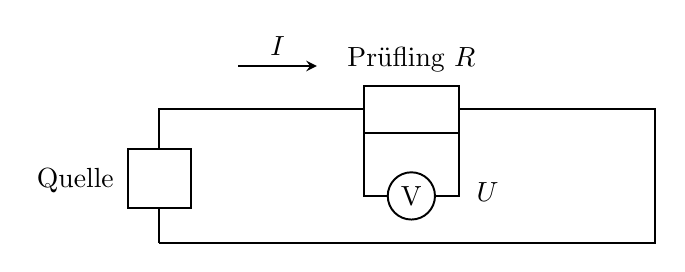
\begin{tikzpicture}[line width=0.7pt,>=stealth]
    \draw (0,0) -- (0,1.7) -- (2.6,1.7);
    \draw (3.8,1.7) -- (6.3,1.7) -- (6.3,0) -- (0,0);
    \draw[fill=white] (-0.4,0.45) rectangle (0.4,1.2);
    \node[left] at (-0.45,0.8) {Quelle};
    \draw[fill=white] (2.6,1.4) rectangle (3.8,2.0);
    \node[above] at (3.2,2.05) {Prüfling $R$};
    \draw[->] (1,2.25) -- (2,2.25) node[midway,above] {$I$};
    \draw (2.6,1.7) -- (2.6,0.6) -- (2.9,0.6);
    \draw (3.5,0.6) -- (3.8,0.6) -- (3.8,1.7);
    \draw[fill=white] (3.2,0.6) circle (0.3);
    \node at (3.2,0.6) {V};
    \node[right] at (3.9,0.65) {$U$};
  \end{tikzpicture}
  \caption[Beispiel einer Versuchsskizze]{Schematischer Beispielaufbau mit
    Quelle, Prüfling und Spannungsmessung. Eigene Darstellung; reale
    Gerätedetails und Strommessung ergänzen.}
  \label{fig:setup}
\end{figure}

\section{Durchführung und Auswertung}
\offen{Arbeitsschritte, Umgebungsbedingungen, Wiederholungen und
Auswertungsverfahren reproduzierbar beschreiben.}
Direkt erfasste Größen und berechnete Werte werden unterschieden.
Für jeden unterschiedlichen Rechenschritt wird ein Zahlenbeispiel gezeigt.
Ergänzende Unterlagen sind in Anhang~\ref{app:records} aufgeführt.
\end{mcimethods}

\chapter{Ergebnisse und Diskussion}
\label{chap:results}

\section{Darstellung der Daten}
In \tabref{tab:example} werden synthetische Beispieldaten zur Demonstration
von Einheiten, Dezimalstellen und Unsicherheiten gezeigt. Die Unsicherheiten
sind hier als Standardunsicherheiten definiert; ihre Werte sind für dieses
Satzbeispiel frei gewählt.
\begin{table}[htbp]
  \centering
  \caption[Synthetische Beispieldaten]{Synthetische Beispieldaten, keine
    Messwerte. $u_U$ und $u_I$ bezeichnen die zugeordneten
    Standardunsicherheiten von Spannung und Stromstärke.}
  \label{tab:example}
  \begin{tabular}{c S[table-format=1.3] S[table-format=1.3]
                    S[table-format=2.2] S[table-format=1.2]}
    \toprule
    Nr. & {$U/\unit{\volt}$} & {$u_U/\unit{\volt}$}
        & {$I/\unit{\milli\ampere}$} & {$u_I/\unit{\milli\ampere}$} \\
    \midrule
    1 & 1.000 & 0.005 & 10.00 & 0.10 \\
    2 & 2.000 & 0.005 & 20.00 & 0.10 \\
    3 & 3.000 & 0.005 & 30.00 & 0.10 \\
    \bottomrule
  \end{tabular}
\end{table}

In \figref{fig:example-plot} werden dieselben Punkte mit horizontalen und
vertikalen Fehlerbalken dargestellt. Die gestrichelte Modellgerade wird
mit dem vorgegebenen Beispielwert $R=\qty{100}{\ohm}$ gezeichnet; sie ist
keine Regression. Die kleinen Fehlerbalken entsprechen den Beispielwerten
und werden nicht künstlich vergrößert.
\begin{figure}[htbp]
  \centering
  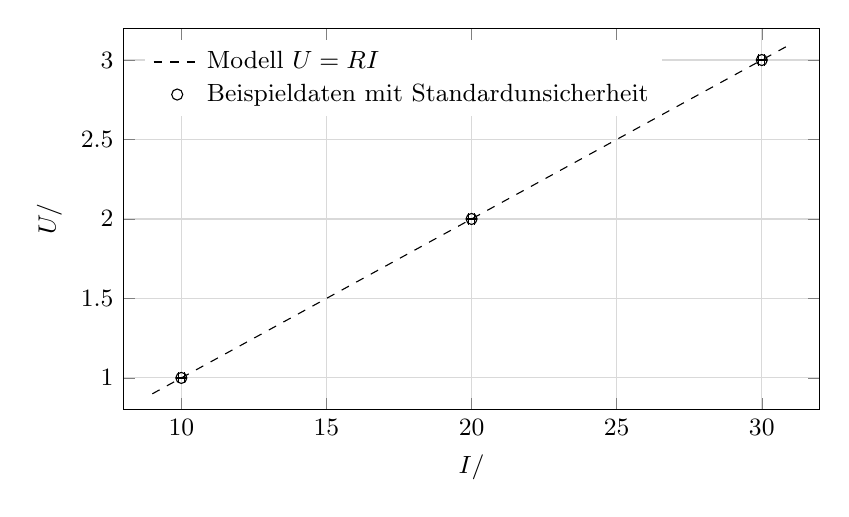
\begin{tikzpicture}
    \begin{axis}[
      width=0.86\linewidth,height=0.53\linewidth,
      xlabel={$I/\unit{\milli\ampere}$},ylabel={$U/\unit{\volt}$},
      xmin=8,xmax=32,ymin=0.8,ymax=3.2,
      xtick={10,15,20,25,30},ytick={1,1.5,2,2.5,3},
      grid=major,grid style={black!15},
      legend pos=north west,legend cell align=left,
      tick label style={font=\small},label style={font=\small},
      legend style={font=\small,draw=none},
    ]
      \addplot[black,dashed,domain=9:31,samples=2] {0.1*x};
      \addlegendentry{Modell $U=RI$}
      \addplot[only marks,mark=o,black,
        error bars/.cd,x dir=both,x explicit,y dir=both,y explicit]
        coordinates {(10,1) +- (0.1,0.005)
                     (20,2) +- (0.1,0.005)
                     (30,3) +- (0.1,0.005)};
      \addlegendentry{Beispieldaten mit Standardunsicherheit}
    \end{axis}
  \end{tikzpicture}
  \caption[Beispieldaten mit Modellgerade]{Synthetische Beispieldaten
    (Kreise mit Fehlerbalken) und vorgegebene Modellgerade (gestrichelt).
    Eigene Darstellung; keine experimentellen Ergebnisse.}
  \label{fig:example-plot}
\end{figure}

\section{Vollständige Beispielrechnung}
Für Zeile 1 in \tabref{tab:example} wird mit \eqnref{eq:ohm} gerechnet:
\begin{equation}
  R = \frac{U}{I}
    = \frac{\qty{1.000}{\volt}}{\qty{10.00e-3}{\ampere}}
    = \qty{100.0}{\ohm}.
  \label{eq:calculation}
\end{equation}
\eqnref{eq:calculation} zeigt Ansatz, eingesetzte Werte und Ergebnis.
Nur für unkorrelierte Eingangsgrößen und bei zulässiger linearer
Unsicherheitsfortpflanzung ergibt sich hier nach \eqnref{eq:uncertainty}
die kombinierte Standardunsicherheit $u_R$ in \unit{\ohm}:
\begin{equation}
  \begin{aligned}
    u_R &= R\sqrt{\left(\frac{u_U}{U}\right)^2
                    +\left(\frac{u_I}{I}\right)^2} \\
        &= \qty{100.0}{\ohm}
           \sqrt{\left(\frac{\qty{0.005}{\volt}}{\qty{1.000}{\volt}}\right)^2
                +\left(\frac{\qty{0.10}{\milli\ampere}}{\qty{10.00}{\milli\ampere}}\right)^2}
         \approx \qty{1.1}{\ohm}.
  \end{aligned}
  \label{eq:uncertainty}
\end{equation}
Damit wird das Beispielergebnis als
$R=\qty{100.0 +- 1.1}{\ohm}$ angegeben. Die Schreibweise bezeichnet hier
die Standardunsicherheit, kein erweitertes Vertrauensintervall.
\offen{Die verwendete Unsicherheitsmethode fachlich belegen und die
Annahmen anhand der realen Messung prüfen.}

\section{Interpretation und Grenzen}
\offen{Reale Ergebnisse mit Erwartungswerten und Literatur vergleichen;
systematische Effekte, Unsicherheiten, Grenzen und mögliche Verbesserungen
diskutieren. Keine Schlussfolgerungen aus den Vorlagendaten übernehmen.}

\chapter{Fazit und Ausblick}
\label{chap:conclusion}

\offen{Fragestellung anhand der tatsächlichen Ergebnisse beantworten und
die Zielerreichung bewerten.}
Es werden die wesentlichen Erkenntnisse zusammengeführt, die Grenzen der
Aussagekraft benannt und gegebenenfalls weitere Untersuchungen abgeleitet.
Neue Messdaten oder neue unbelegte Aussagen werden hier nicht eingeführt.


\printbibliography[heading=bibintoc,title={\MCIText{Quellenverzeichnis}{References}}]
\MCIPrintBackMatter%
\addchap{\MCIText{Formelzeichenübersicht}{List of symbols}}
% One row per base symbol; do not repeat u_U, u_I, u_R as separate variants.
\begin{longtable}{@{}p{0.12\textwidth}p{0.57\textwidth}p{0.23\textwidth}@{}}
  \toprule
  \MCIText{Zeichen}{Symbol} & \MCIText{Bedeutung}{Description}
    & \MCIText{Einheit}{Unit} \\
  \midrule
  \endhead
  $I$ & Elektrische Stromstärke & \unit{\ampere} \\
  $R$ & Elektrischer Widerstand & \unit{\ohm} \\
  $U$ & Elektrische Spannung & \unit{\volt} \\
  $u$ & Standardunsicherheit einer Größe; Einheit wie Bezugsgröße
      & \unit{\ampere}, \unit{\ohm} oder \unit{\volt} \\
  \bottomrule
\end{longtable}
\noindent Es werden keine physikalischen Konstanten im Vorlagenbeispiel
verwendet. \offen{Bei Bedarf verwendete physikalische Konstanten mit
Wert, Einheit und Quelle ergänzen.}

\appendix
\chapter{Ergänzende Unterlagen}
\label{app:records}

\offen{Rohdaten, Versuchsprotokoll, ergänzende Rechnungen oder relevante
Auszüge der Aufgabenstellung ergänzen.}
Der Anhang wird im Haupttext an der passenden Stelle referenziert,
beispielsweise als Anhang~\ref{app:records}. Externe Unterlagen erhalten
einen Quellenverweis. Die römische Seitenzählung wird aus dem vorderen
Dokumentteil fortgesetzt.

\end{document}
